\documentclass[12pt]{amsart}
\usepackage[T1]{fontenc}
\usepackage[utf8]{inputenc}

\usepackage[top=1.95cm, bottom=1.95cm, left=2.35cm, right=2.35cm]{geometry}

\usepackage{hyperref}
\usepackage{enumitem}
\usepackage{tcolorbox}
\usepackage{float}
\usepackage{cleveref}
\usepackage{multicol}
\usepackage{fancyvrb}
\usepackage{amsmath}
\usepackage[french]{babel}
\usepackage[
    type={CC},
    modifier={by-nc-sa},
	version={4.0},
]{doclicense}

\newcommand\floor[1]{\left\lfloor #1 \right\rfloor}

\usepackage{tnsmath}
\usepackage{tnsalgo}


\newtheorem{fact}{Fait}[section]
\newtheorem{example}{Exemple}[section]
\newtheorem{remark}{Remarque}[section]
\newtheorem*{proof*}{Preuve}

\setlength\parindent{0pt}

\floatstyle{boxed} 
\restylefloat{figure}


\DeclareMathOperator{\taille}{\text{\normalfont\texttt{taille}}}

\newcommand\sqseq[2]{\fbox{$#1$}_{\,\,#2}}


\DefineVerbatimEnvironment{rawcode}%
	{Verbatim}%
	{tabsize=4,%
	 frame=lines, framerule=0.3mm, framesep=2.5mm}
	 
	 
	 
\begin{document}

\title{BROUILLON - Des opérations (pas si) simples}
\author{Christophe BAL}
\date{20 Octobre 2020}

\maketitle

\begin{center}
	\itshape
	Document, avec son source \LaTeX, disponible sur la page
	
	\url{https://github.com/bc-writing/drafts}.
\end{center}


\bigskip


\begin{center}
	\hrule\vspace{.3em}
	{
		\fontsize{1.35em}{1em}\selectfont
		\textbf{Mentions \og légales \fg}
	}
			
	\vspace{0.45em}
	\doclicenseThis
	\hrule
\end{center}


\bigskip
\setcounter{tocdepth}{2}
\tableofcontents


% ------------- %


\newpage

\section{Multiplication efficace avec Alexevich Karatsuba}

	\subsection{Une petite histoire dans la grande}
	À l'automne 1960, lors d'un séminaire organisé par Kolmogorov, ce dernier parla de la conjecture suivante :
\emph{\og Une multiplication de deux nombres de $n$ chiffres ne peut être réalisée en moins de $\bigO(n^2)$ opérations élémentaires \fg}.

\medskip

Karatsuba, qui avait assisté au séminaire, mit une semaine pour proposer une méthode en $\bigO(n^{\lg 3})$ opérations élémentaires
\footnote{
	La fonction $\lg$ désigne le logarithme binaire c'est à dire celui en base $2$.	
},
contredisant ainsi le grand Kolmogorov
\footnote{
	Il semblerait que Kolomogorov ait été très secoué par cette découverte, voire vexé.
	En effet, en 1962 Kolmogorov écrivit un article, sans doute avec Yuri Ofman l'un de ses élèves, sans en informer Karatsuba qui n'apprit l'existence de l'article que plus tard, lors de sa réédition. 
}.
Nous allons présenter cet algorithme en le redécouvrant de façon très \og naturelle \fg.



	\subsection{Multiplier efficacement deux grands nombres}
	Comment calculer efficacement le produit $p = 12\,345\,678 \cdot 87\,654\,321$ , c'est à dire en faisant le moins de multiplications possibles ?

\medskip

La 1\iere{} idée de la méthode de Karatsuba est de procéder comme suit.

\begin{enumerate}
	\item 
	\begin{explain}[style = sar]
		p
			\explnext{}
		(1\,234 \cdot 10^4 + 5\,678) \, (8\,765 \cdot 10^4 + 4\,321)
			\explnext{}
		1\,234 \cdot 8\,765 \cdot 10^8
		+ (1\,234 \cdot 4\,321 + 5\,678 \cdot 8\,765) \cdot 10^4
		+ 5\,678 \cdot 4\,321)
	\end{explain}
	
	\item On procède alors de façon analogue pour chaque nouveau produit \emph{(nous allons voir que Karatsuba a été très malin pour gérer cette étape)}. Concentrons-nous juste sur $q = 1\,234 \cdot 8\,765$ par exemple.
	 
	\leavevmode\kern-1.75em
	\begin{explain}[style = sar]
		q
			\explnext{}
		(12 \cdot 10^2 + 34) \, (87 \cdot 10^2 + 65)
			\explnext{}
		12 \cdot 87 \cdot 10^4
		+ (12 \cdot 65 + 34 \cdot 87) \cdot 10^2
		+ 34 \cdot 65
	\end{explain}
	
	\item Il reste alors des \og dernières \fg{} étapes du type suivant en considérant $r = 12 \cdot 65$.
	 
	\leavevmode\kern-1.75em
	\begin{explain}[style = sar]
		r
			\explnext{}
		(1 \cdot 10 + 2) \, (6 \cdot 10 + 5)
			\explnext{}
		1 \cdot 2 \cdot 10^2
		+ (1 \cdot 6 + 2 \cdot 6) \cdot 10
		+ 2 \cdot 5
	\end{explain}
\end{enumerate}


\medskip


Les habitués de l'algorithmique reconnaissent ici une approche de type \og diviser pour mieux régner \fg. Pour simplifier nous allons considérer des nombres à $n = 2^k$ chiffres quitte à rajouter des zéros inutiles à gauche.
La 1\iere{} idée consiste donc à considérer
$(a \cdot 10^{n/2} + b) \, (A \cdot 10^{n/2} + B)$
via
$a \cdot A \cdot 10^n + (a \cdot B + A \cdot b) \cdot 10^{n/2} + b \cdot B$
où
$(a ; b ; c ; d) \in \ZintervalC{0}{10^{n/2} - 1}$.


\bigskip


Essayons de voir si l'on peut éviter de faire le calcul de tous les 4 produits $a \cdot A$ ,  $a \cdot B$ , $b \cdot B$ et $b \cdot A$ . 
Pour cela nous allons prendre un peu de recul
\footnote{
	L'auteur de ces notes ne sait pas ce qui a réellement guidé Karatsuba dans sa découverte.
}
en considérant le polynôme $P(X) = (a \cdot X + b) \, (A \cdot X + B)$ et posons $P(X) = c_2 \cdot X^2 + c_1 \cdot X + c_0$ . Projetons-nous alors un peu plus loin pour avancer...

\begin{enumerate}
	\item $c_0 = P(0)$ c'est à dire $c_0 = b \cdot B$ .

	
	\item $c_2 = a \cdot A$ peut être vue comme la valeur à l'infini du polynôme $P$. Si l'on reste dans le cadre réel, on peut penser à un équivalent en $+\infty$. On peut en fait donner une définition très algébrique en considérant l'homogénéisé
	\footnote{
		Ce genre de considération est naturelle quand l'on fait de la géométrie projective.
		Le point $(1 ; 0)$ est un point à l'infini du plan projectif.
	}
	de $P$ qui est par définition le polynôme $P_h(X ; T) = c_2 \cdot X^2 + c_1 \cdot X \cdot T + c_0 \cdot T^2$ .
	Dès lors, nous avons : $P_h(1 ; 0) = c_2$ .

	
	\item
	\begin{explain}[style = sar, ope = \iff]
		P(1) = c_2 + c_1 + c_0
			\explnext{}
		c_1 = P(1) - c_2 - c_0
			\explnext{}
		c_1 = (a + b) \, (A + B) - c_2 - c_0
	\end{explain}
	
	
	\item En résumé, 
	$c_0 = b \cdot B$ ,
	$c_2 = a \cdot A$
	et surtout 
	$c_1 = (a + b) \, (A + B) - c_2 - c_0$ .
	Donc il suffit de calculer les trois produits
	$c_0 = b \cdot B$ ,
	$c_2 = a \cdot A$
	et 
	$(a + b) \, (A + B)$,
	pour avoir au passage $c_1$ ,
	puis d'utiliser
	$(a \cdot X + b) \, (A \cdot X + B) %
	 = %
	 c_2 \cdot 10^n + c_1 \cdot 10^{n/2} + c_0$ .
	Joli ! Non ?
\end{enumerate}


\begin{remark}
	On aurait aussi pu considérer $P(-1)$, ce qui donne :
	
	\smallskip
	
	\begin{explain}[style = sar, ope = \iff]
		P(-1) = c_2 - c_1 + c_0
			\explnext{}
		c_1 = c_2 + c_0 - P(-1)
			\explnext{}
		c_1 = c_2 + c_0 - (a - b) \, (A - B)
	\end{explain}
	
	\smallskip
	
	L'intérêt de la formule précédente est que le produit $(a - b) \, (A - B)$ est moins grand en valeur absolue que $(a + b) \, (A + B)$
	\emph{(nous donnons une application de ceci dans la section suivante)}.
	
	\smallskip
	
	On pourrait vouloir passer via $P(k)$ où $k \in \ZZ$. Ceci semble a priori peu prometteur car on obtient alors $c_1 = c_2 \, k^2 + c_0 - (a + k \, b) \, (A + k \, B)$ et inutile pour nous car là nous devons faire plus de produits que les deux méthodes ci-dessus.
\end{remark}



	\subsection{Un petit détour du côté du produit de deux entiers à deux chiffres}
	
Avec $n = 2$, nous avons une façon originale de faire le produit de deux entiers à deux chiffres. Considérons par exemple le produit $56 \cdot 78$. Voici ce que donne la méthode de Karatsuba dans ce cas.
	
\begin{enumerate}
	\item Ici $a = 5$ , $b = 6$ , $A = 7$ et $B = 8$ .

	\item $c_2 = 5 \cdot 7 = 35$ .

	\item $c_0 = 6 \cdot 8 = 48$ .

	\item $c_1 = (5 + 6) \, (7 + 8) - 35 - 48 = 165 - 35 - 48 = 82$ .

	\item $56 \cdot 78 = c_2 \cdot 10^2 + c_1 \cdot 10^1 + c_0 = 3500 + 820 + 48 = 4368$ .
\end{enumerate}
	
\medskip
	
Visuellement nous avons fait les calculs suivants où $c_0$ et $c_2$ sont des multiplications \og verticales \fg{} et $c_1$ s'obtient en soustrayant ces deux multiplications au produit des \og additions horizontales \fg{}.
	
\begin{center}
	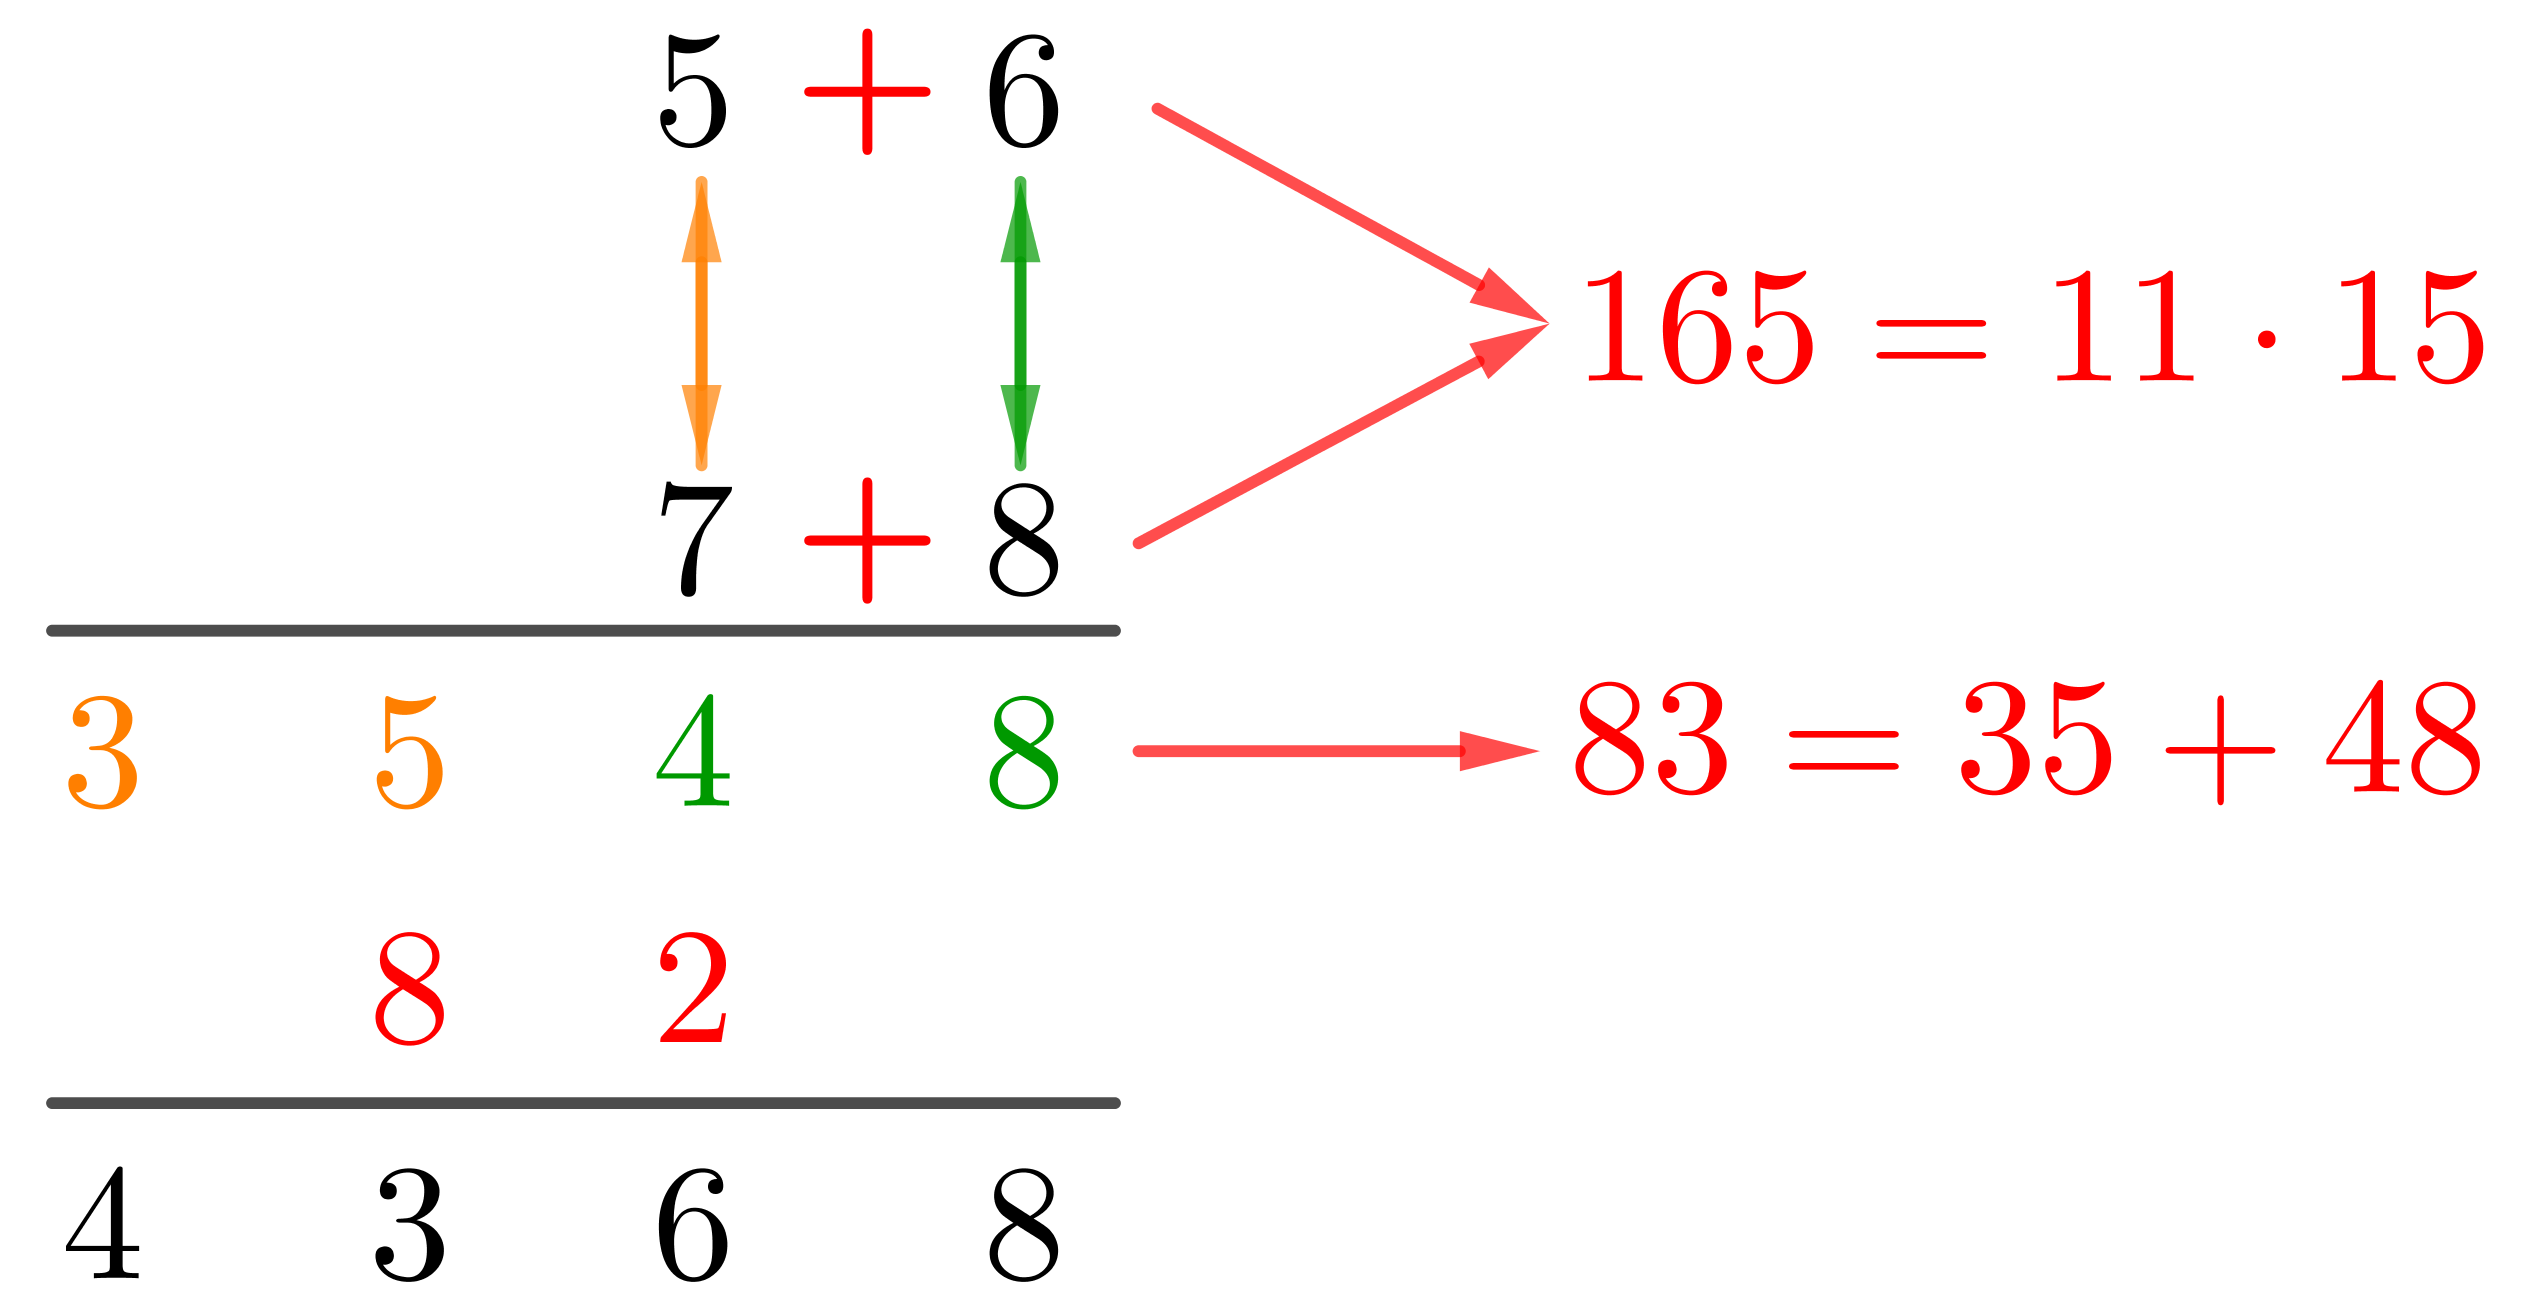
\includegraphics[scale=.75]{not-so-basic-arithmetic-ope/product-two-digits-karatsuba.png}
\end{center}

\medskip

Notons que le calcul directement via
$a \cdot A \cdot 10^2 + (a \cdot B + A \cdot b) \cdot 10 + b \cdot B$
donne une méthode plus utile pour un calcul mental sans crayon ni papier car les calculs se font au fil de l'eau de la droite vers la gauche avec peu de calculs intermédiaires à retenir.
	
\begin{center}
	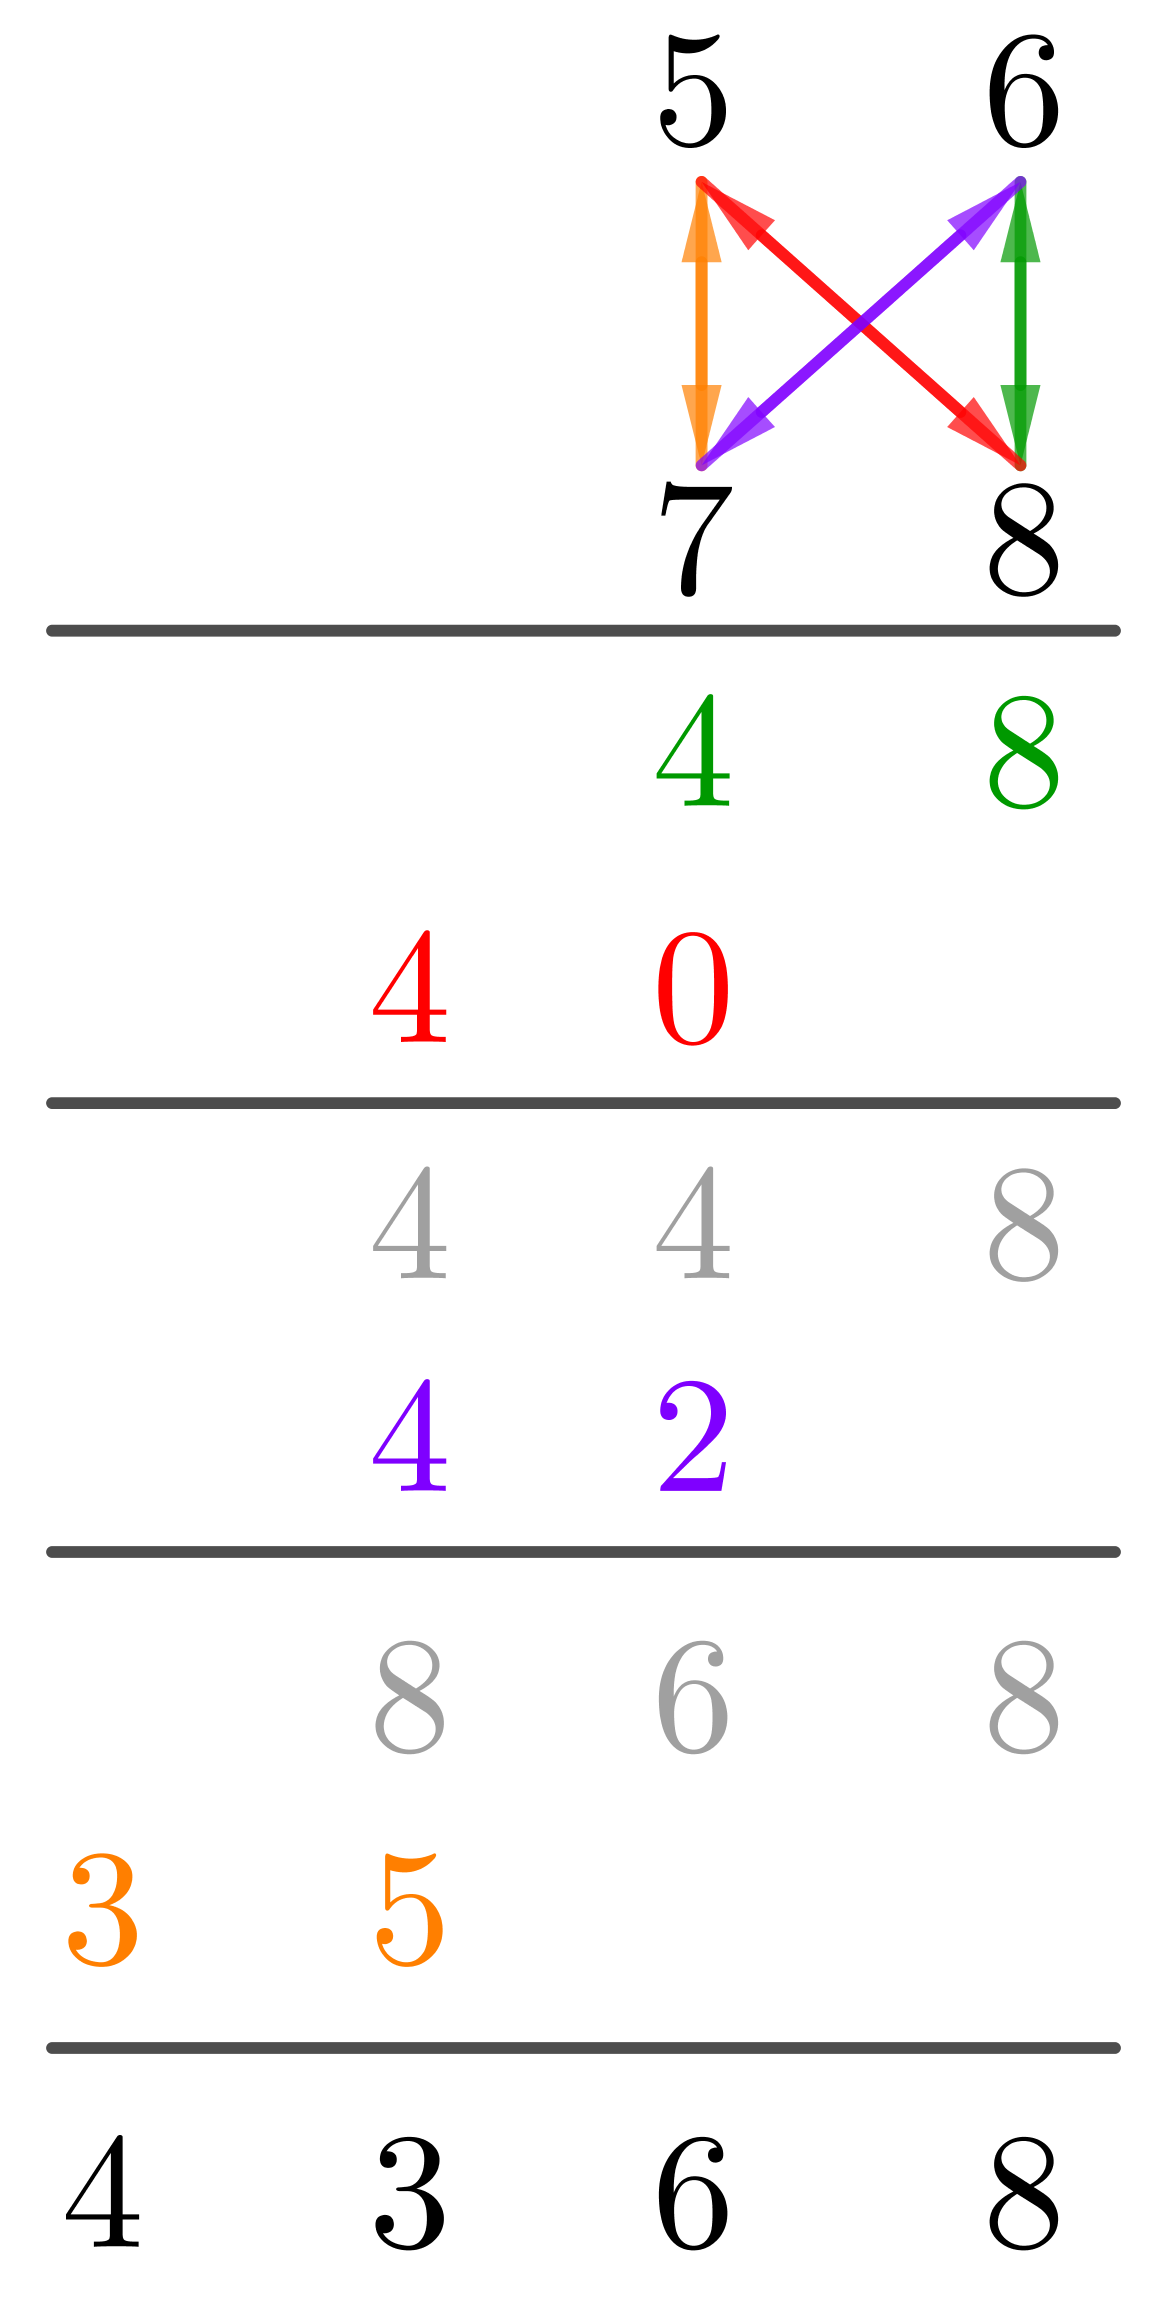
\includegraphics[scale=.75]{not-so-basic-arithmetic-ope/product-two-digits-easier.png}
\end{center}


%	\subsection{Complexité algorithmique}
%	\input{not-so-basic-arithmetic-ope/product-karatsuba-complexity}


\end{document}
